\section{Controller Subsystem}

% Why the MCU connects to the internet
In order for our system to be as self and power efficient as possible from an end-user perspective, our team decided to use a low-power, Internet-of-Things (IoT)-focused wireless microcontroller. To make the process of operating our product as hands-off as possible to end-users, the microcontroller will operate in Access Point (AP) mode to serve information to the user's mobile device. Our product will not produce or receive large amounts of data, or need complicated control schema for our various subsystems---and with power budget being a major concern of ours, our team needed to choose a product that would fit the bill.

% How the MCU connects to the internet (local network, LAN -> NAT -> WAN, TCP stack)
\subsection{CC3220 Overview}
The Texas Instruments CC3220-series (hence referred to as the "CC3220", the "MCU", or the "microcontroller") of microcontrollers are WiFi-enabled chips with an ARM Cortex-M4 central processor and a WiFi network processor, along with many useful peripherals and power management modules. This series of processors is delivered alongside a software development kit (SDK) provided by Texas Instruments to ease the development of IoT applications. The CC3220 is capable of running on bare metal, or with a Real-time Operating System (RTOS), allowing us to organize and schedule our various tasks.

The CC3220's WiFi network processor (NWP) supports 802.11b/g/n, SmartConfig provisioning, IPv4 and IPv6. The NWP also as the ability to host an internal HTTP/HTTPS server, and contains its own filesystem.

\subsection{Connection}
Our product shall be able to broadcast a WLAN in AP mode. This will allow the user to connect to the product's SSID. The user would then be directed to a web portal hosted by the MCU's internal HTTP server, where they will be able to view information and telemetry related to the product. Hosting a web interface would allow unanimous adaptation of our product for home users. The system shall be able to broadcast a WLAN in AP mode with a nominal signal strength of 6 dBm measured at the antenna. The network shall adhere to the standards of 802.11b, g, or n. 

% Parameters for connection and how often it tries
\subsection{Weather API Implementation}
As a stretch goal, the user will be able to configure the MCU in Station mode to allow it to connect to the user's home WLAN's SSID as a client. The user would still be able to access the MCU's web portal and see the same information as they had before. In addition, the MCU would be able to access an API to receive weather information and inform the user of recommended actions pertaining to their garden bed (e.g. if the system determines there will be freezing temperatures overnight, it may suggest to the user to cover the garden bed with a sheet or towel).

% Any over-the-air updates?
\subsection{Over-the-Air Updates}
At this time, our team does not intend to provide a method for over-the-air updates (OTA), however, this is a stretch goal that may be completed in the future.

\subsection{Startup and Shutdown} Startup and shutdown will occur in a timely manner (within seconds). Abrupt shutdown shall not damage any components of the system, and the system will be able to restart to its previous state without any input from the user. If the system freezes or crashes, its internal watchdog timer will automatically reboot the device.

\subsection{Data} As well as being able to see and configure the network settings of the product, the user will be able to see data relating to the OH-levels and common plant nutrient levels as determined by the spectral analysis of the product. For one measurement, our team will need to store 16 bits of data per position from 130 unique positions, per sensor.
\begin{equation}
    \frac{16\,\mathrm{b}}{8\,\mathrm{b/B}}\times 130\,\mathrm{positions} \times 2\,\mathrm{sensors} = 520\,\mathrm{B}
\end{equation}
With 8 Mb of the 32 Mb (1 MiB of the 4 MiB) shared serial flash dedicated to storing results, this allows us to store 2016 measurements.
\begin{equation}
    \frac{1\,\mathrm{MiB}}{520\,\mathrm{B/measurement}} = 2016\,\mathrm{measurements}
\end{equation}
Stretching out measurements to be recorded every 15 minutes, this will allow a user to see individual measurements stretching back exactly three weeks.
\begin{equation}
    2016\,\mathrm{measurements} \times \frac{1\,\mathrm{measurement}}{15\,\mathrm{min}} = 30240\,\mathrm{min} 
\end{equation}
As a stretch goal these measurements can be aggregated and analyzed, and allow us to serve trends and predictions to the user.

\subsection{Low Power Modes} The system shall run in active mode between sunrise and sunset, while the battery has 40-100\% calculated charge remaining. The system shall run in low power mode between sunrise and sunset while the battery has 10-40\% calculated charge remaining, and between sunset and sunrise while the battery has 10-100\% calculated charge remaining. The system shall run in critical power mode while the battery has 5-10\% calculated charge remaining. The system shall be in shutdown mode while the battery has 0-5\% calculated charge remaining. The system shall be able to switch power modes within 5 seconds of the interrupt being triggered.

% Libraries
\subsection{Libraries}
It should be expected that the C++ standard library (as defined in C++14) will be used, as well as the POSIX library, along with the Texas Instruments SimpleLink CC32xx SDK.

\subsection{Sensing} The system shall monitor and perform analog-to-digital conversion of the spectral values sensor values at least every 15 minutes while in active mode. The system will use I2C to talk to the analog-to-digital converter (ADC) located in the sensing subsystem. 

\subsection{Motor Control} Four GPIO lines will be used to control the stepper motor holding the sensing PCB (which includes the photodiodes, op-amp circuitry, ADC, motor controller, and connector). Depending on the digital values passed to the motor controller, the motor controller is able to control the movement direction and speed. Our team found that using the SimpleLink SDK's high-level hardware abstraction layer (HAL) provides too long of a delay when changing values in the four GPIO lines. Nanosecond-levels of delay were needed, rather than the microsecond levels of delay our team was seeing. Instead of using highly-abstracted APIs for control of the motor, our team got as close to hardware as is possible with C/C++ and used TI's driverlib driver library specifically for the CC3220. Instead of a simple GPIO number being passed to the function, our team had to determine the GPIO port and port-specific pin of each input of our motor controller. The driverlib function checks the port for correctness, and then performs a system call to write a value directly to memory (in our case, the address of the GPIO port). Using driverlib also allows us to bit stuff our GPIO pins if they are located on the same port---in our second iteration of the board, the motor controller GPIOs were relocated to the same GPIO port and bitmasks used so we can change all four GPIO pins with one driverlib write function. This allows us to toggle a single GPIO pin within a period of 350 ns (seen in \ref{fig:gpio_toggle_driverlib}). With a speed of 80 MHz in active mode, this would mean we're able to write to GPIO in only 28 processor cycles.
\begin{equation}
    350\,\mathrm{ns} \times (80\times10^6\mathrm{cycles/s}) = 28\,\mathrm{cycles}
\end{equation}
This is a huge accomplishment for our team, especially with a program written in C++ and utilizing HAL.

\begin{figure}
    \centering
    \label{fig:gpio_toggle_driverlib}
    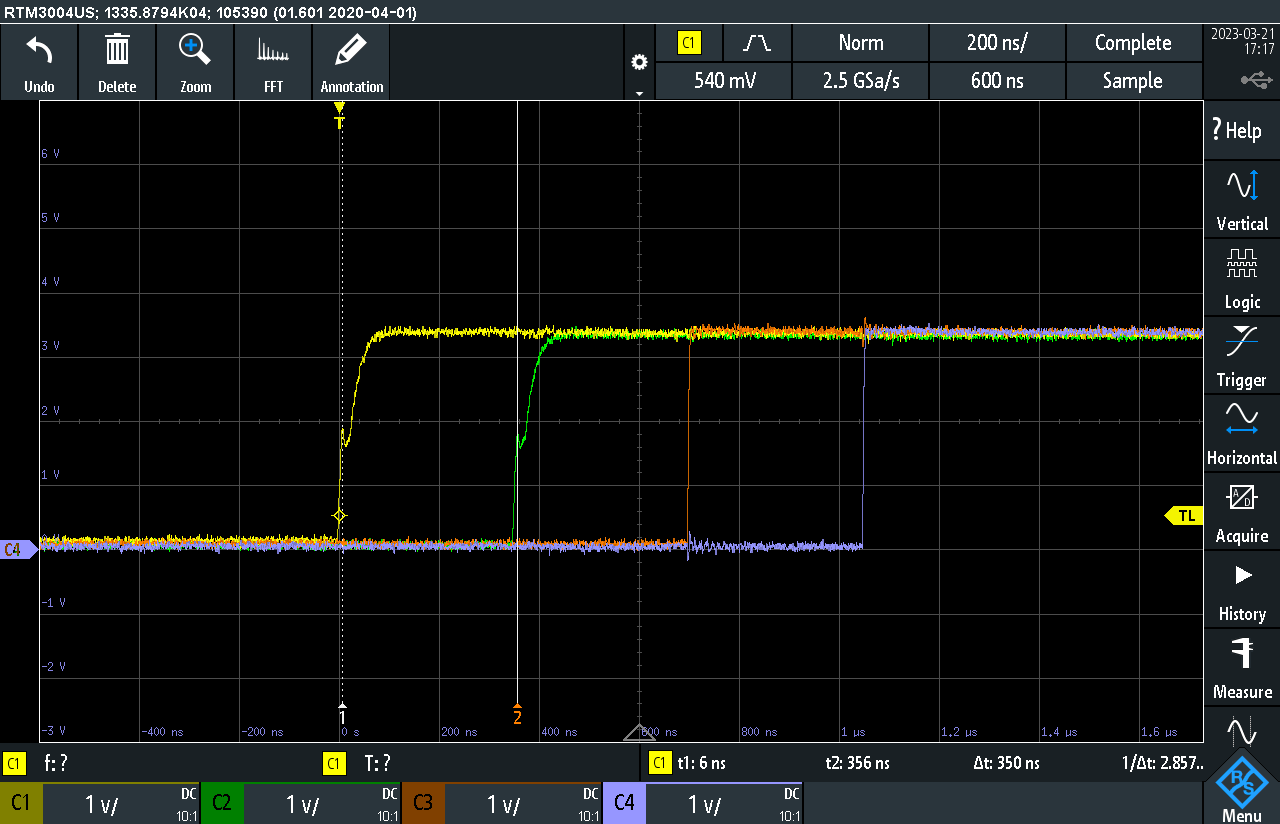
\includegraphics[width=\linewidth]{images/gpio_toggle_driverlib.jpg}
    \caption{Toggling GPIO using driverlib results in a very short (350 ns) delay.}
\end{figure}

% How the MCU gets data from sensors (ADC)
\subsection{Analog-to-digital Conversion}
The sensing subsystem contains a Texas Instruments ADS 7142 ADC. The ADS 7142 is an IoT-focused nanowatt ADC with 2 external channels, an I2C interface, a sampling frequency of 140ksps, and an effective resolution of 16 bits in High-precision Mode. This ADC will be able to measure between 0 and 3.3 V from the output of the sensing subsystem's  photodiode op-amp circuit.

% How the MCU gets data from sensors (ADC, cont.)
It is expected that each photodiode's circuit will provide a voltage of between 0 and 3.3 V. The 16-bit ADC provides for an input of the same range. Therefore, the resolution of the ADC is calculated below:
\begin{equation}
    \frac{(3.3 - 0)\,\mathrm{V}}{2^{16}\,\mathrm{steps}} =
    50.35\,\mathrm{\mu V}/\mathrm{step}
\end{equation}
These steps will be used to measure OH composition and nutrients in the soil. The MCU will directly control GPIO and bit-bang values to the stepper motor controlling the position of the photodiodes allowing them to measure the full range of spectral values.

% What kind of development model?
\subsection{Development Model}
An Agile development model was used to program the control subsystem and its various modules. Code reviews were performed on an as-needed basis by a convening of members of the MCU subsystem and the web subsystem teams. Texas Instruments Code Composer Studio v12 was used to program, compile (via TI ARM compiler v20), and debug the C++-based project. GitHub was used as a repository for the project, using GNU Git for version control.

The Meyers' Singleton design pattern was used for most of the classes found in our project repository (e.g. for our water solenoid class as seen in \ref{fig:singleton_implementation}). Because our team is using a RTOS with a scheduler and threads, we are using that to our advantage to divide and schedule tasks for the different submodules of our project. However, one problem our team took into consideration is that there is was only one physical instance of each submodule. The normal Singleton pattern traditionally has been used when one wants only one instance of a class initialized at any one point, but they are not thread-safe. One variation of this pattern is the Meyers' Singleton, which guarantees that only one instance of a type is available at any time. Initialization of this pattern is thread-safe, and locks can be used to ensure thread safety when accessing members of the class. This is accomplished by using a static local variable inside a static member function to hold a single instance of the class. The Meyers' Singleton takes advantage of the fact that the initialization of static local variables inside functions is guaranteed to be thread-safe. The Meyers' Singleton disallows copying and moving of the class, and makes member constructors and destructors private.

% Code style
\lstdefinestyle{mystyle}{
    basicstyle=\ttfamily\footnotesize,
    breakatwhitespace=false,         
    breaklines=true,                 
    captionpos=b,                    
    keepspaces=true,                 
    numbers=left,                    
    numbersep=-15pt,                  
    showspaces=false,                
    showstringspaces=false,
    showtabs=false,                  
    tabsize=2
}
\lstset{style=mystyle}

\begin{figure}
    \centering
    \label{fig:singleton_implementation}

\begin{lstlisting}[language=C++]
    class Water { 
        public:
            static Water& instance();

            // Disallow copying
            Water& operator = (const Water&) = delete;
            Water(const Water&) = delete;

            // Disallow moving
            Water& operator = (Water&&) = delete;
            Water(Water&&) = delete;

            // Class functions
        
        private:
            Water();
            ~Water();

            // Class variables
    };
\end{lstlisting}
\caption{An example of the Meyers' Singleton pattern implementation within the project.}
\end{figure}

% Power
\subsection{Power}
The MCU will receive regulated 3.3, 5, and 12 V power from from the power subsystem. This power will be routed to various modules and other subsystems.

% LEDs
\subsection{LEDs} The system shall be able to make use of its onboard LEDs for notifying the user or developers of system states. When the system is in active mode, the green LED shall be solidly illuminated. When the system is in low power mode, the green LED shall flash 1 time for a period of 0.5 seconds, every 2 seconds. When the system is in critical power mode, the red LED shall flash 2 times for a period of 0.5 seconds per flash, seperated by 1 second between each flash, every 30 seconds. When the system is in shutdown mode, no LEDs shall be active. When the system is starting up, the green and red LED shall be solidly illuminated until the startup sequence is completed and the system transitions into a different power mode.

% PCB
\subsection{Printed Circuit Board} Our controller subsystem was developed and implemented on a Texas Instruments LaunchPad development board. An initial control printed circuit board (PCB) was designed, fabricated, and assembled (partially seen in \ref{fig:mcu_v1_cpwg}). The chip version of the CC3220 (CC3220S) was used requiring a 4-layer impedance-controller PCB, with waveguide and external antenna, as well as oscillators, numerous bypass capacitors, and inductors. A revised PCB was designed using the module version of the CC3220 (CC3220MODAS). The PCB design was simplified, requiring only a few bypass capacitors instead of the numerous other components to support the microcontroller found on the first revision of the board.

\begin{figure}
    \centering
    \label{fig:mcu_v1_cpwg}
    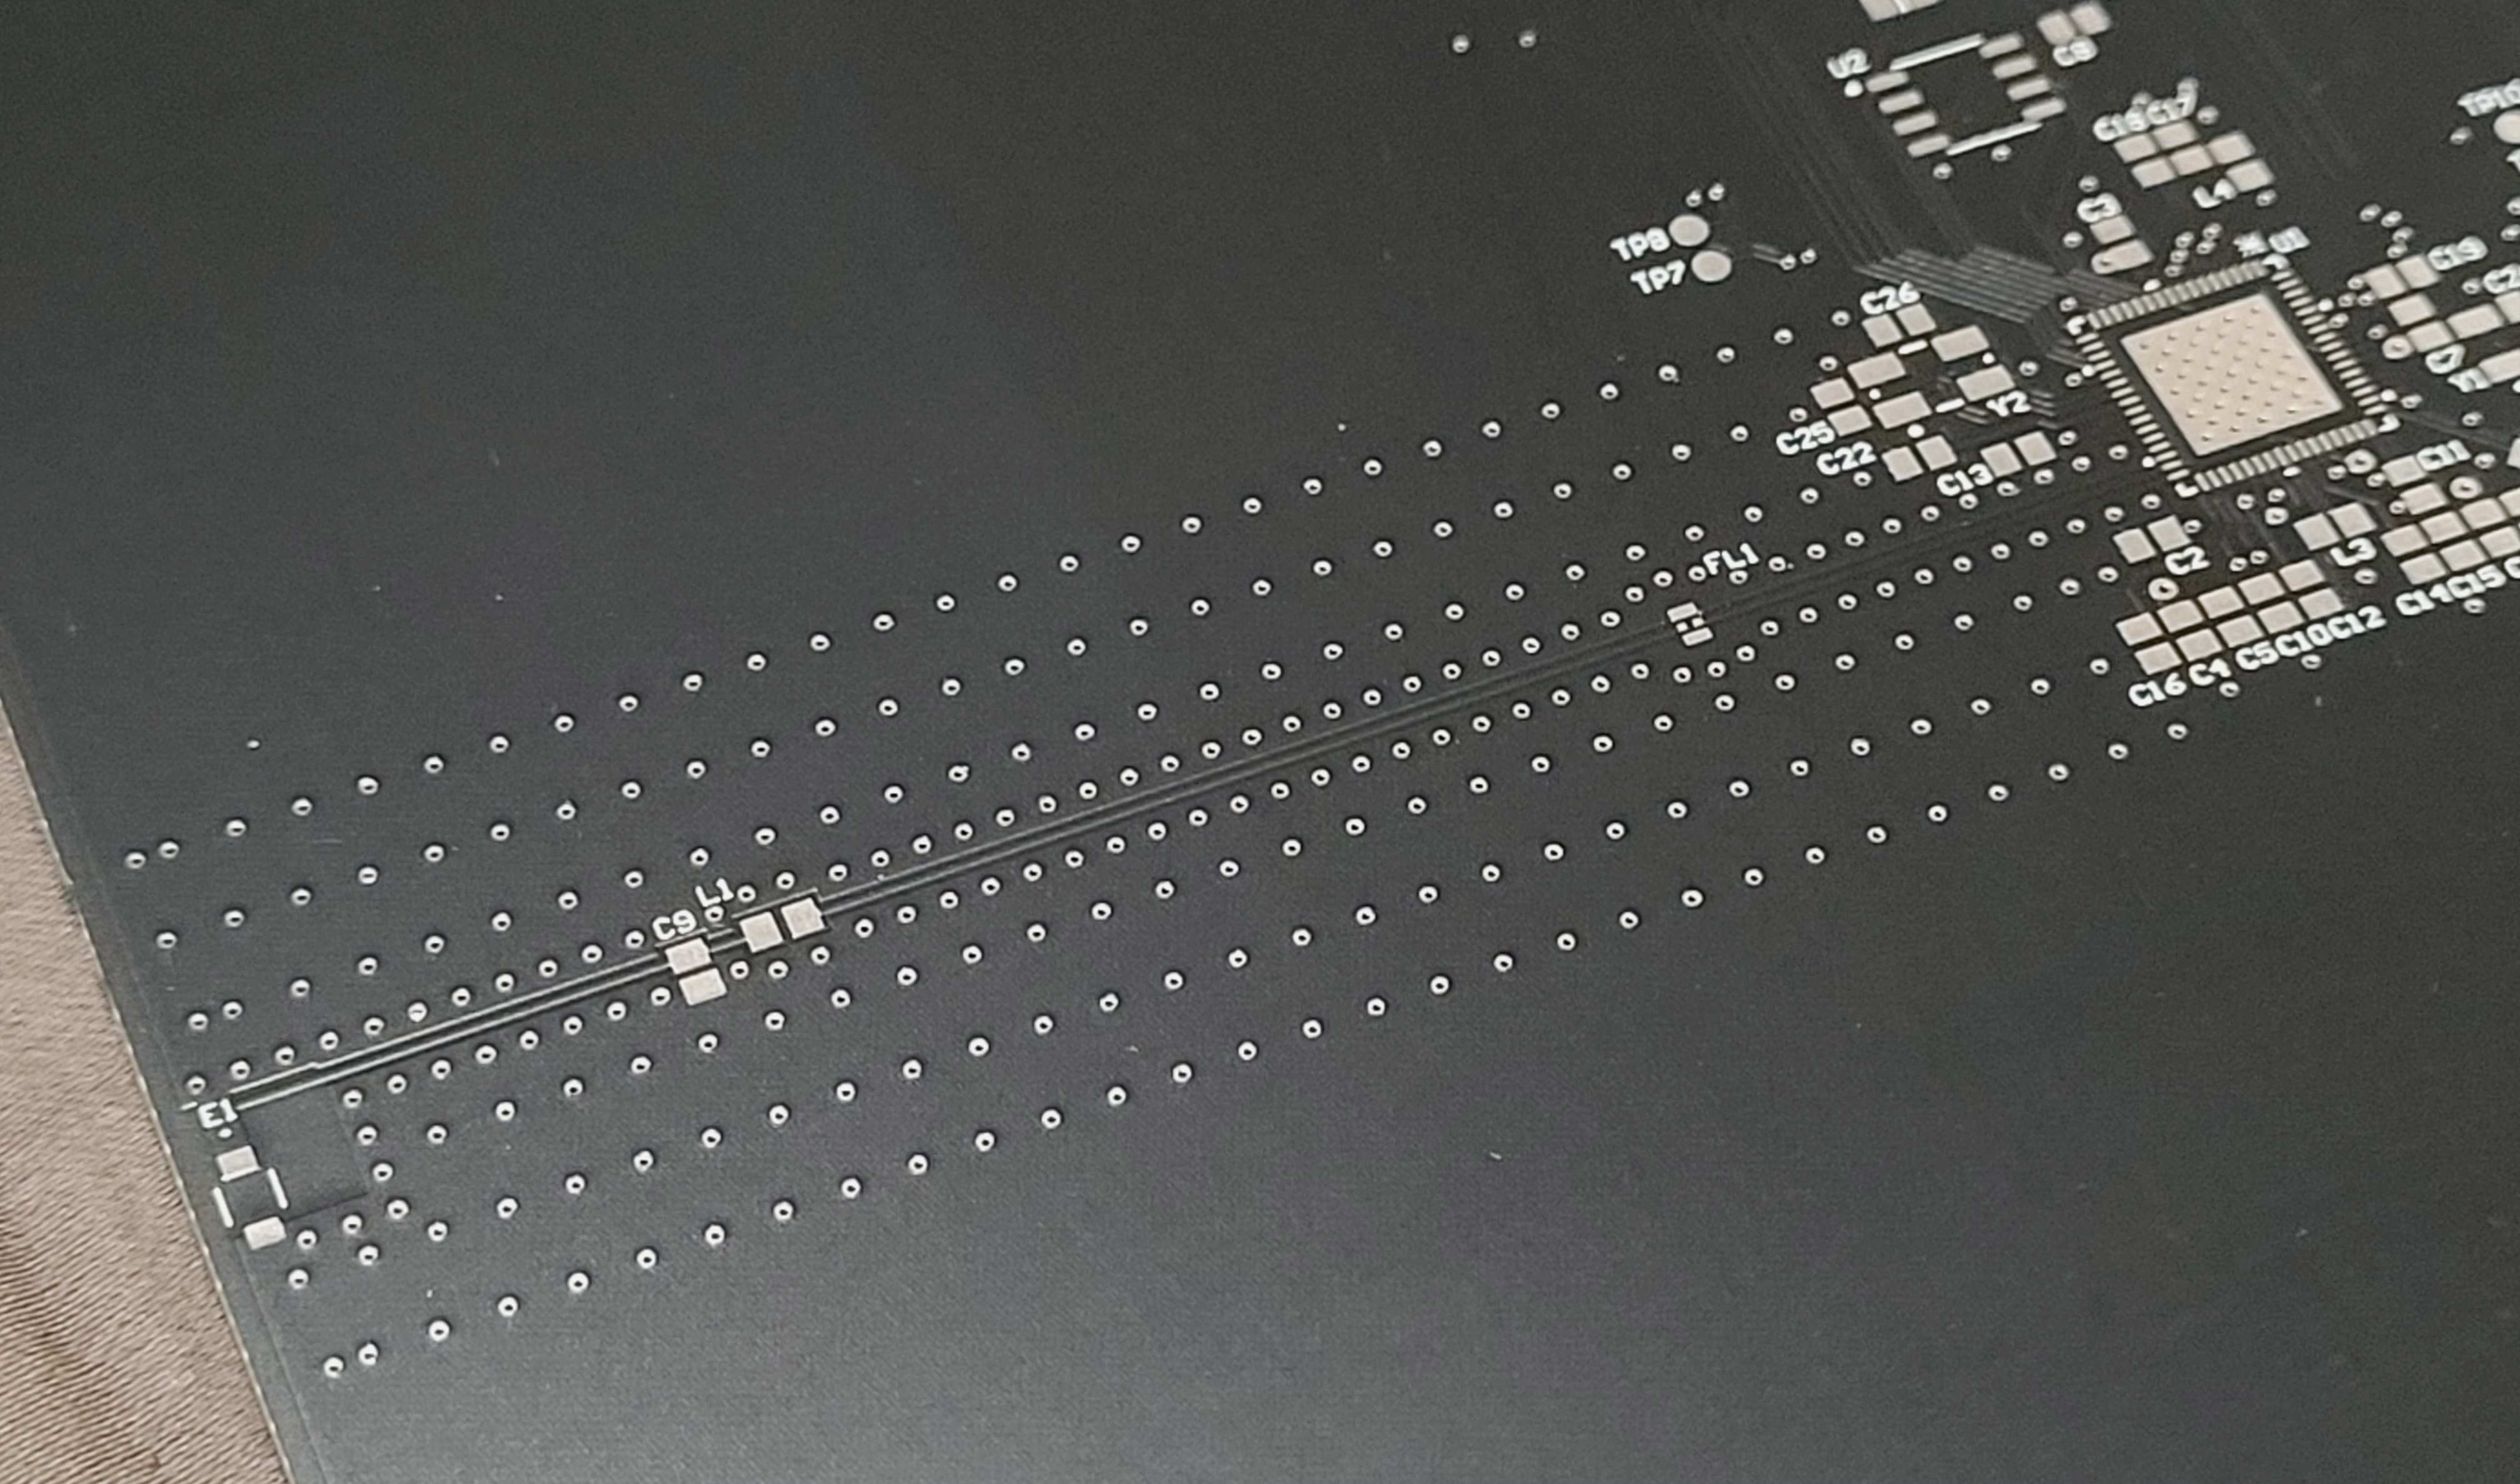
\includegraphics[width=\linewidth]{images/mcu_v1_cpwg.jpg}
    \caption{The coplanar waveguide designed to carry a 2.4 GHz signal surrounded by via fencing.}
\end{figure}